
% \subsection{Setup}
% \begin{figure}
%   \centering
%   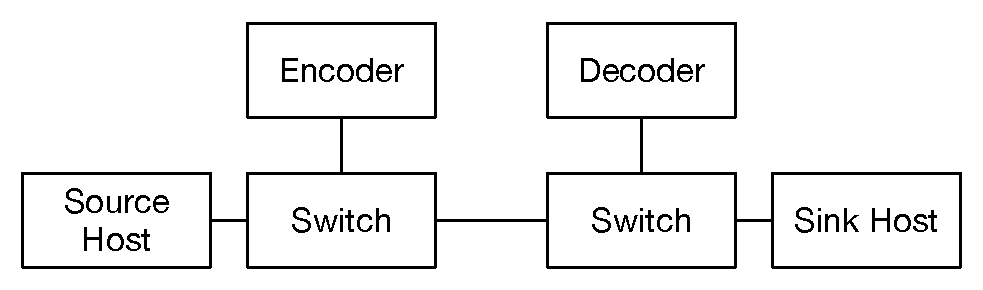
\includegraphics[width=0.3\paperwidth]{exp_topo.pdf}
%   \caption{\label{fig:exp_topo} Testbed topology for benchmarks.}
% \end{figure}

% Figure~\ref{fig:exp_topo} depicts the testbed we used to benchmark \OurSys.
% \hg{This setup was not used to test the FPGA, so it probably does not
% belong in a section on its own.}
% The two traffic generation hosts are each connected to different \OurSys
% enabled switches, which are themselves connected by a 10 GbE link. The
% switches are Wedge BF32-100X's with Barefoot Tofino~\cite{tofino} P4 
% programmable forwarding engines. \lei{TODO: fix cite}


\begin{figure}
  \centering
  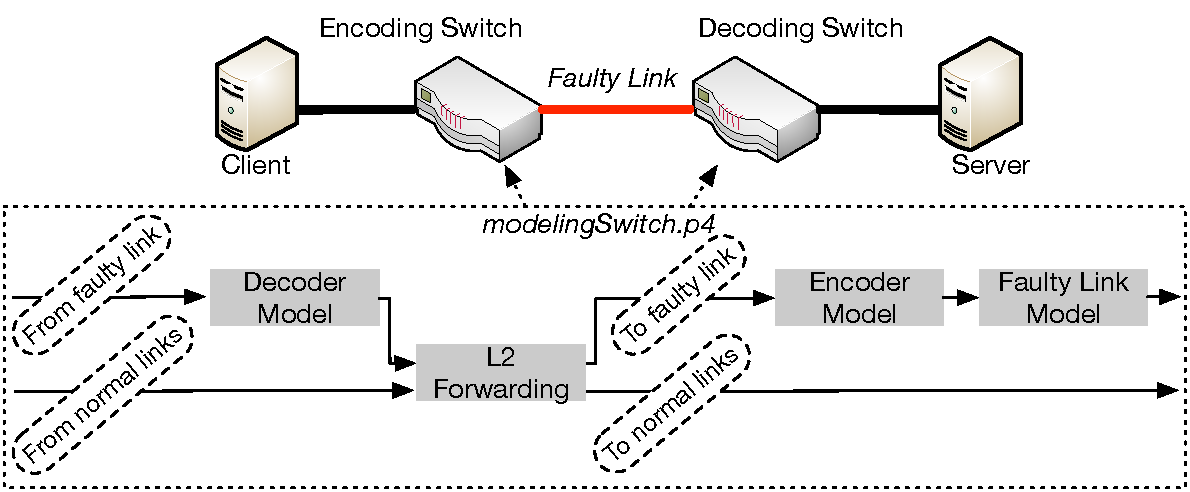
\includegraphics[width=0.4\paperwidth]{figures/lineRateModel.pdf}
  \caption{\label{fig:p4ModelTopo} Topology of the 10 Gb/s testbed 
  for real-time TCP benchmarks, using P4 to model FEC and faulty links.}
\end{figure}

To measure the effect of faulty links and \OurSys at the protocol and
application level, we developed a P4 pipeline for the Barefoot Tofino that
models \OurSys. We deployed the model in the testbed network shown in
Figure~\ref{fig:p4ModelTopo} and ran end-to-end Iperf benchmarks on it in
real-time. The P4 pipeline models the behavior of faulty links and FEC,  and
can be reconfigured via the control plane at runtime.

% of the encoder,  decoder, and
% faulty link, and can be reconfigured with different FEC and  packet loss
% parameters at runtime via the control plane.

The \textbf{encoder model} of the pipeline encapsulates each packet egressing on
the faulty link with the \OurSys header and inserts blank  parity packets into
the flow.
%It tracks per-port block IDs and  packet indices using P4 register
%arrays. To generate parity packets, the  model clones the last data packet in
%each block with the Tofino's multicast engine.

The \textbf{faulty link model} adds a \emph{corruption header} to each packet
egressing the faulty link. The header indicates whether or not the neighbor
switch should consider the packet lost. The model selects packets for
corruption according to a simple binomial distribution implemented with the
Tofino's random number generator.

Finally, the \textbf{decoder model} processes packets ingressing from  the
faulty link. It removes the corruption and \OurSys headers  and passes non-
corrupt packets to forwarding. It withholds corrupt packets, using
recirculation, until the block ends. If it has counted at least K data plus
parity packets in the block, the model "recovers" all of the corrupt packets
by allowing them to pass to forwarding; else, the model drops the corrupt
packets.

All experiments we describe below measure performance of 10 second file
transfers from the client to the server, through an encoding switch, faulty
link, and decoding switch. We ran 25 trials for each tested configuration of
K, H,  and loss rate.


\begin{figure*}[!ht]
\centering
\begin{minipage}[b]{0.32\linewidth}
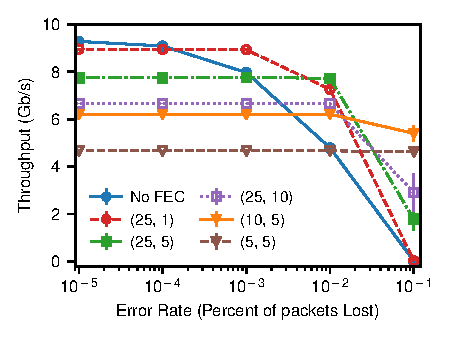
\includegraphics[width=\linewidth]{figures/lossVsTput.pdf}
\caption{Iperf throughput.}
\label{fig:lossVsTput}
\end{minipage}
\hspace{.05in}
\begin{minipage}[b]{0.32\linewidth}
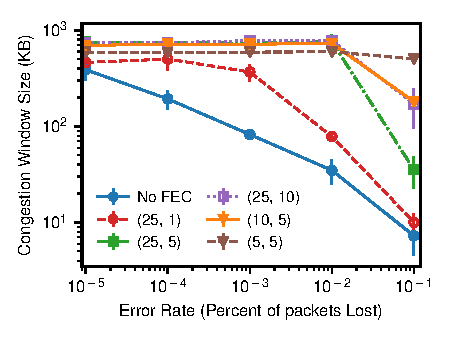
\includegraphics[width=\textwidth]{figures/lossVsWindow.pdf}
\caption{Iperf TCP window sizes.}
\label{fig:lossVsWindow}
\end{minipage}
\hspace{.05in}
\begin{minipage}[b]{0.32\linewidth}
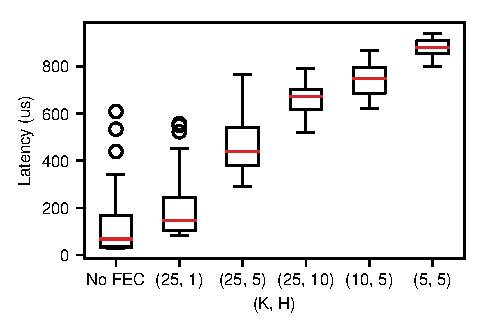
\includegraphics[width=\textwidth]{figures/latency.pdf}
\caption{Network latency.}
\label{fig:latency}
\end{minipage}
\end{figure*}

% \begin{figure}
%   \centering
%   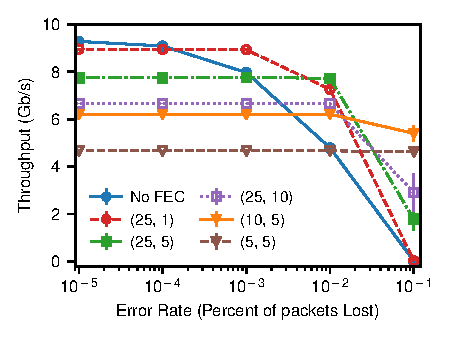
\includegraphics[width=0.3\paperwidth]{figures/lossVsTput.pdf}
%   \caption{\label{fig:lossVsTput} Iperf throughput at different loss rates.}
% \end{figure}

% \begin{figure}
%   \centering
%   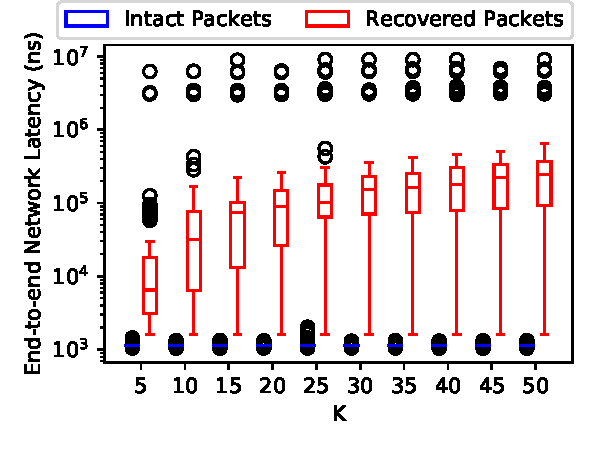
\includegraphics[width=0.3\paperwidth]{figures/udpLatency.pdf}
%   \caption{\label{fig:lossVsLatencyUdp} Network latency for a 100 Mb/s UDP flow (H = 5, loss rate = $10 ^{-2}$).}
% \end{figure}

% \begin{figure}
%   \centering
%   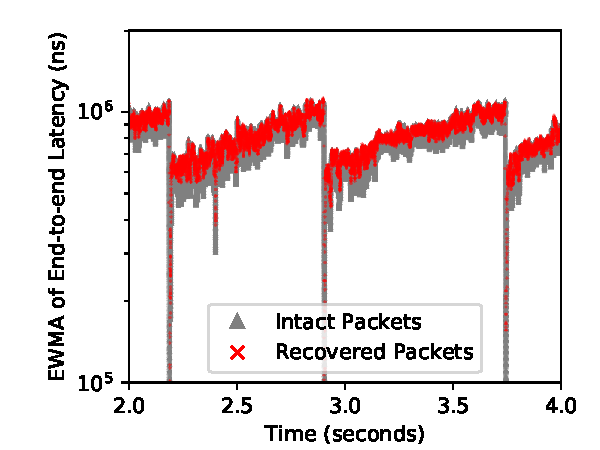
\includegraphics[width=0.3\paperwidth]{figures/tcpLatency.pdf}
%   \caption{\label{fig:lossVsLatencyTcp} Network latency for a 9 Gb/s TCP flow (K = 25, H = 5, loss rate = $10 ^{-2}$).}
% \end{figure}


%Congestion window size ($cwnd$) determines how much data the sender 
%can transmit before receiving an ACK, limiting the transmission rate 
%to approximately $cwnd$ * round trip time.
%TCP increases $cwnd$ linearly 
%with successful packet deliveries, and reduces it exponentially upon 
%packet loss.


Figure~\ref{fig:lossVsTput} shows TCP throughput with different FEC
configurations as loss rate varied. With \OurSys, Iperf sustained  over 5 Gb/s
with loss up to $10^{-1}$ (1 out of every 10 packets dropped). Without
\OurSys, Iperf's throughput at that loss rate was under 25 Mb/s. 

Figure~\ref{fig:lossVsWindow} shows average congestion window size ($cwnd$) in the
trials. Random packet loss at rates higher than $10^{-5}$ caused TCP to
reduce $cwnd$ significantly, resulting in the throughput drop in
Figure~\ref{fig:lossVsTput}. With FEC, $cwnd$ remains high as
loss rate increases, especially when using high levels of redundancy, e.g.,
$(K, H) = (5, 5)$.

Figure~\ref{fig:latency} shows the in-network latency, i.e., from the  ingress
pipeline of the encoding switch to the egress pipeline of the  decoding
switch, in trials with no loss. FEC added under 1ms of average latency in  all
trials. Latency was proportional to $H/K$, because the parity packets
increased the average length of the egress queue to the faulty port by
approximately that factor. TCP adjusts to higher latency  by increasing
$cwnd$, which explains why $cwnd$ increases with ($H/K$) in
Figure~\ref{fig:lossVsWindow}.



% % This figure shows the impact of H. 

% Figure~\ref{fig:lossVsTput} also shows the bandwidth overhead of  FEC, which
% is dominated by the number of parity packets per block ($H$).  At loss rates
% greater than or equal to $10^{-4}$ the bandwidth overhead of adding  parity
% packets had less of an impact on TCP throughput than lost packets, for  most
% configurations tested. To reduce bandwidth overhead, the FEC  can be tuned for the
% loss rate of each specific link, which is reportedly stable over
% time~\cite{corropt}.



% % This figure shows the impact of K.

% To understand how FEC impacts latency, we measured the latency  between the
% ingress pipeline from the source server and the egress pipeline  to the sink
% server, using the nanosecond precision  timestamps of the Tofino, with packets
% routed back through the first  switch before egressing to the sink.
% Figure~\ref{fig:lossVsLatencyUdp}  plots an EWMA of latency for packets in a
% 100 Mb/s UDP flow. For  intact packets, latency was low because they did not
% invoke  the decoder. For  recovered packets, however, the decoder increased
% latency. Average  latency increased with block size because  recovery requires
% the decoder to wait until all the parity packets  for a block arrive. The
% maximum observed latency for recovered packets  was high, around 9 MS. This
% was due to the behavior of the iperf  UDP generator, which periodically paused
% for up to 9 MS between  sending packets, to meet the 100 Mb/s target. The high
% inter-packet  arrival time stalled the generation of parity packets and thus
% the  recovery of any lost packets in the same block.
% \lei{\#Shrink Candidate\#}

% Figure~\ref{fig:lossVsLatencyTcp} plots a time series of latency EWMA  for TCP
% packets in a single maximum rate flow (around 9 Gb/s). The difference in
% latency between recovered versus intact packets was almost indistinguishable.
% Latency for all packets was not dominated by the decoder, but instead by time
% spent  in egress buffers in the switch, which repeatedly filled due to TCPs
% congestion  control dynamics, i.e., causing the familiar ``sawtooth'' pattern
% in Figure~\ref{fig:lossVsLatencyTcp}. Additionally, the latency for packet
% recovery was lower with the TCP workload because average packet rate was
% around 1 order of magnitude higher.



